% Bagian Lampiran
\section*{Lampiran} % Jika ada lampiran

\begin{figure}[htbp]
  \centering
  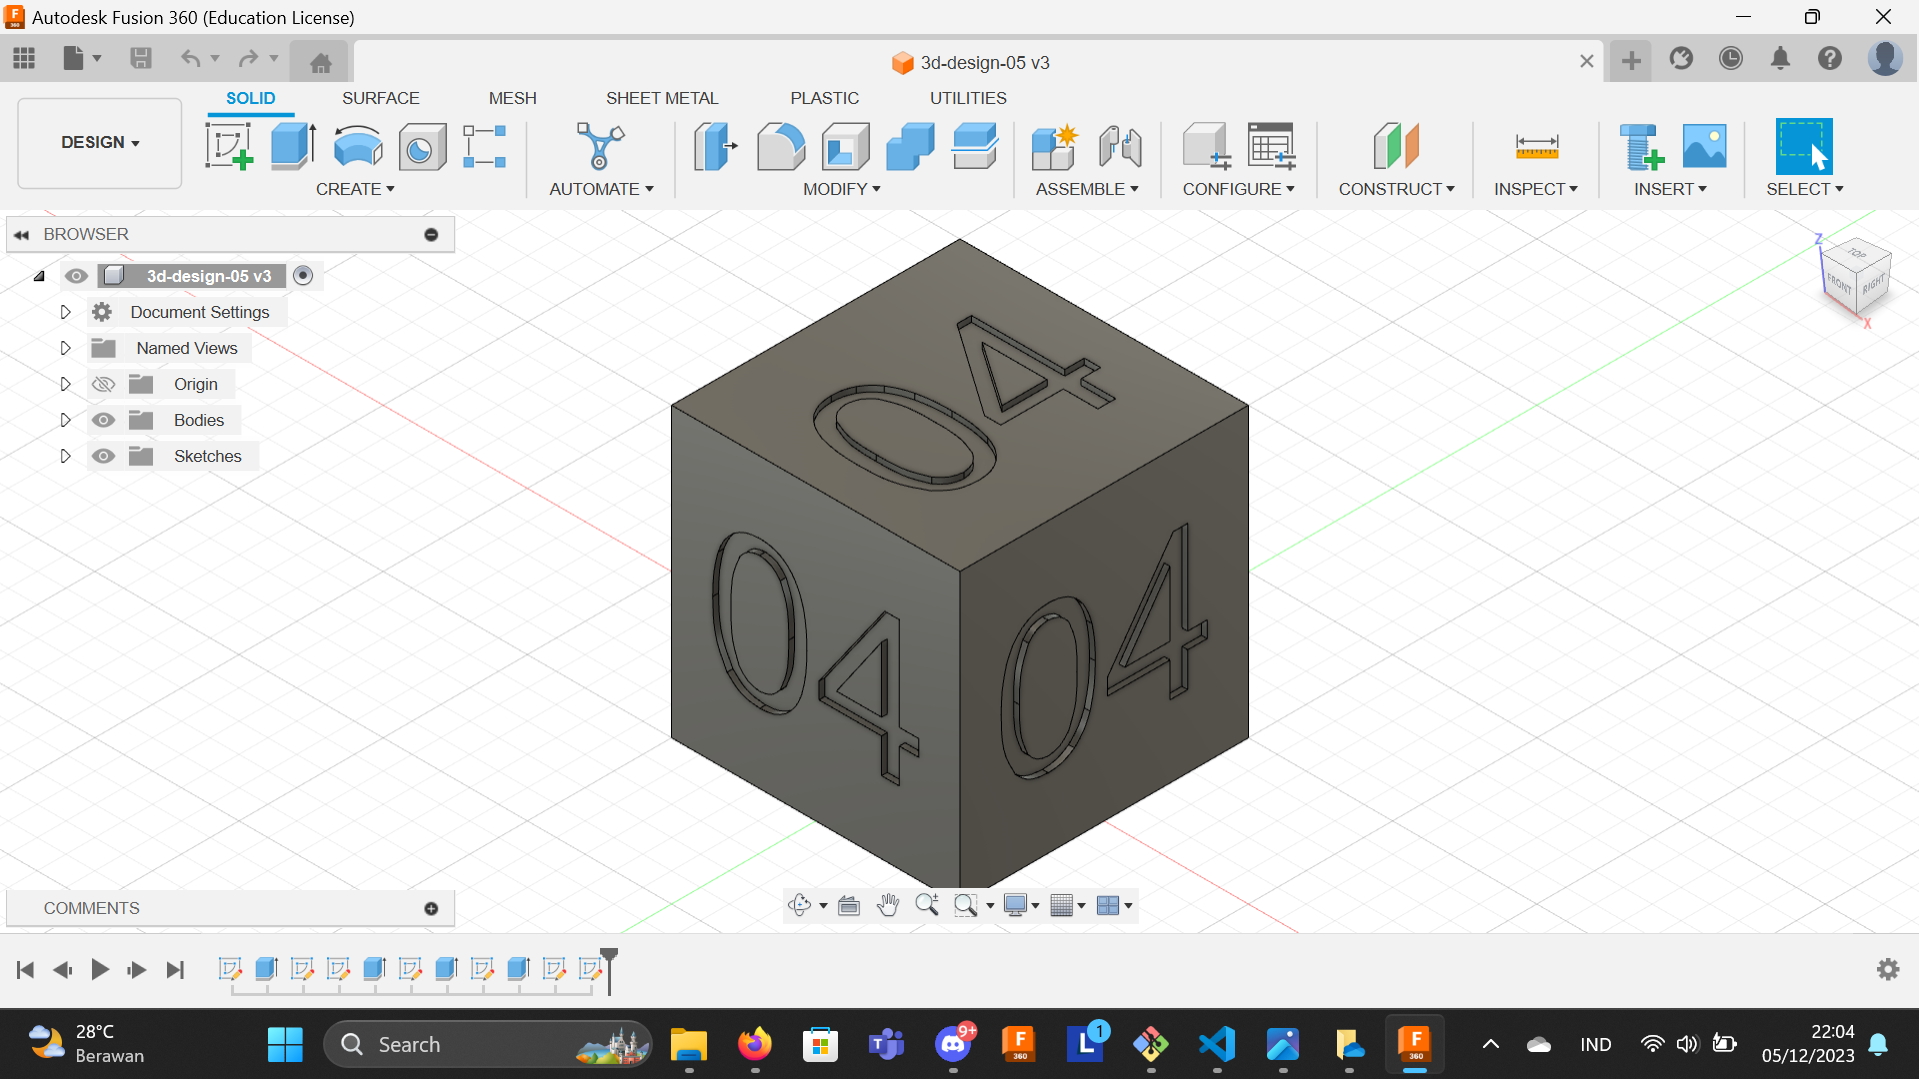
\includegraphics[width=0.8\linewidth]{img/kubus.png}
  \caption{Desain kubus dengan nomor kelompok 4} 
  \label{fig:cube}
\end{figure}

\begin{figure}[htbp]
  \centering
  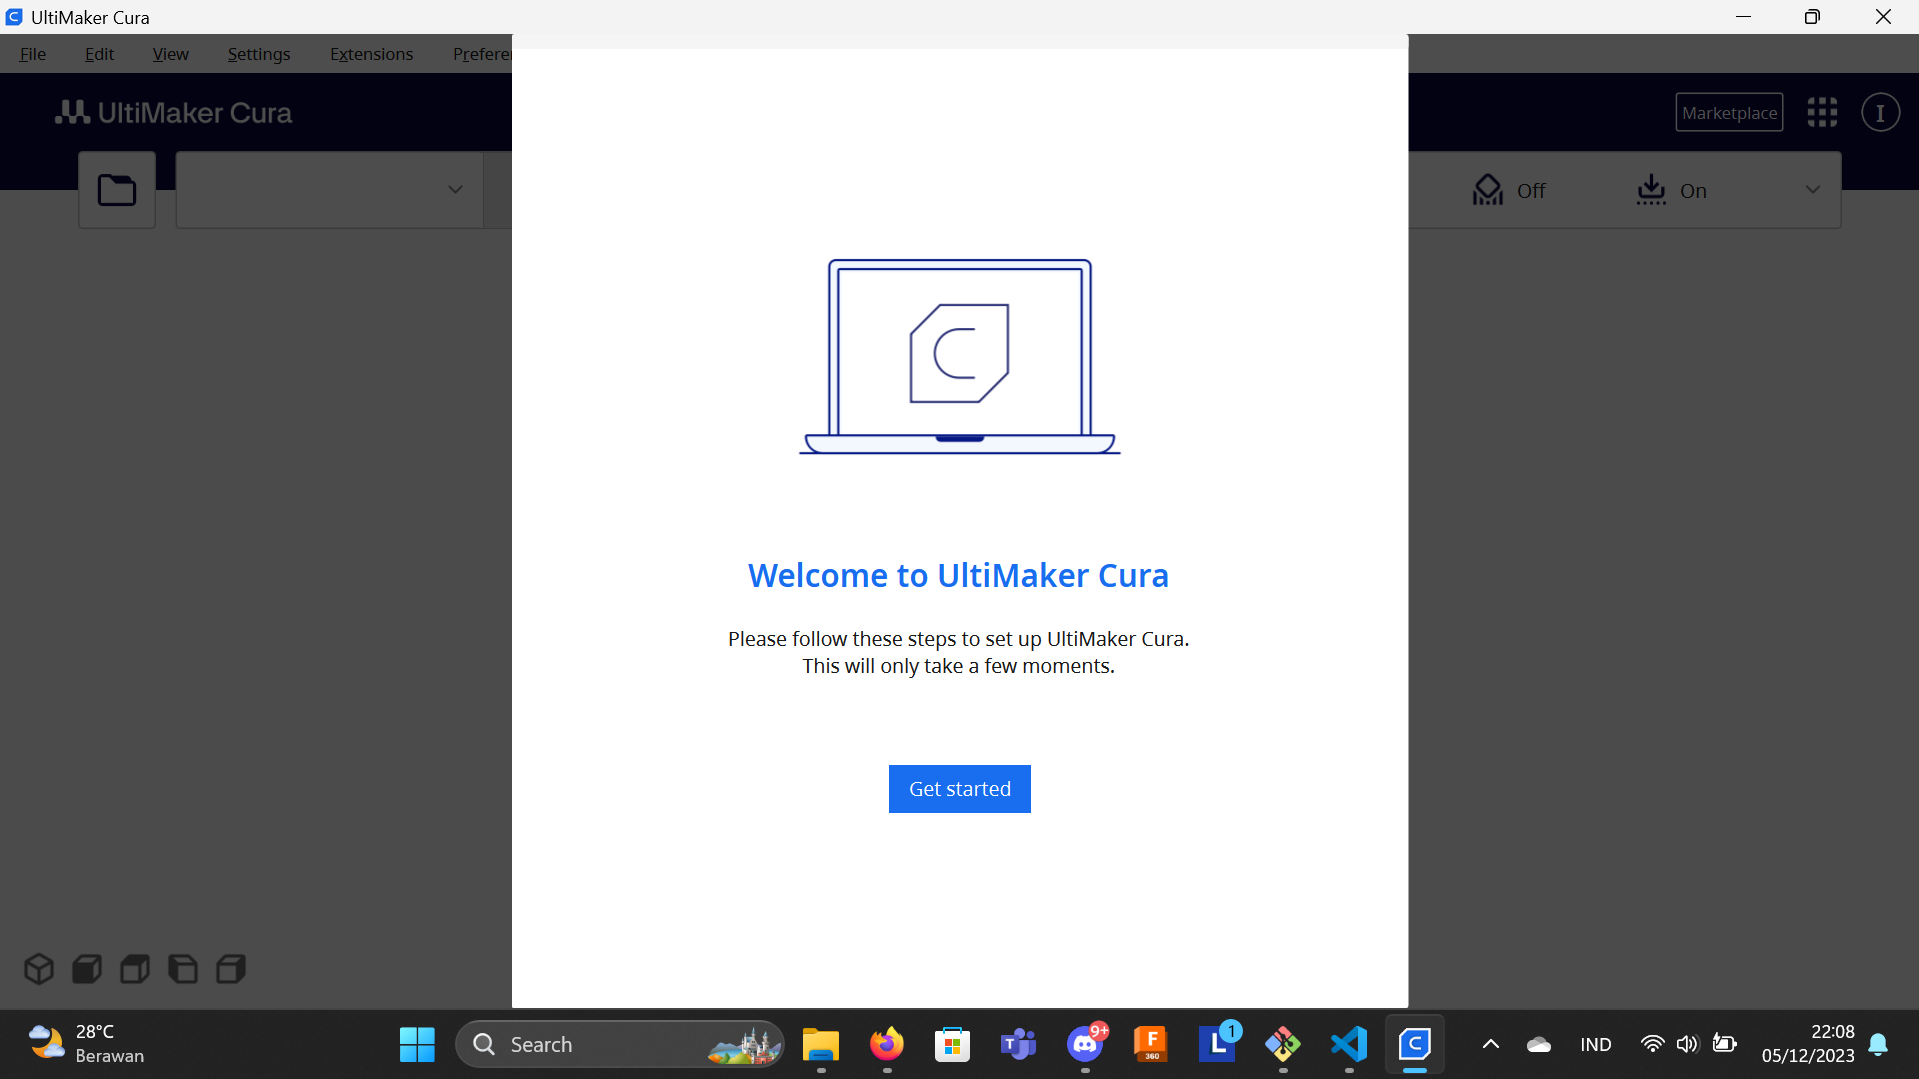
\includegraphics[width=0.8\linewidth]{img/ultimaker.png}
  \caption{Bukti instalasi Ultimaker CURA} 
  \label{fig:ultimaker}
\end{figure}

\begin{figure}[htbp]
  \centering
  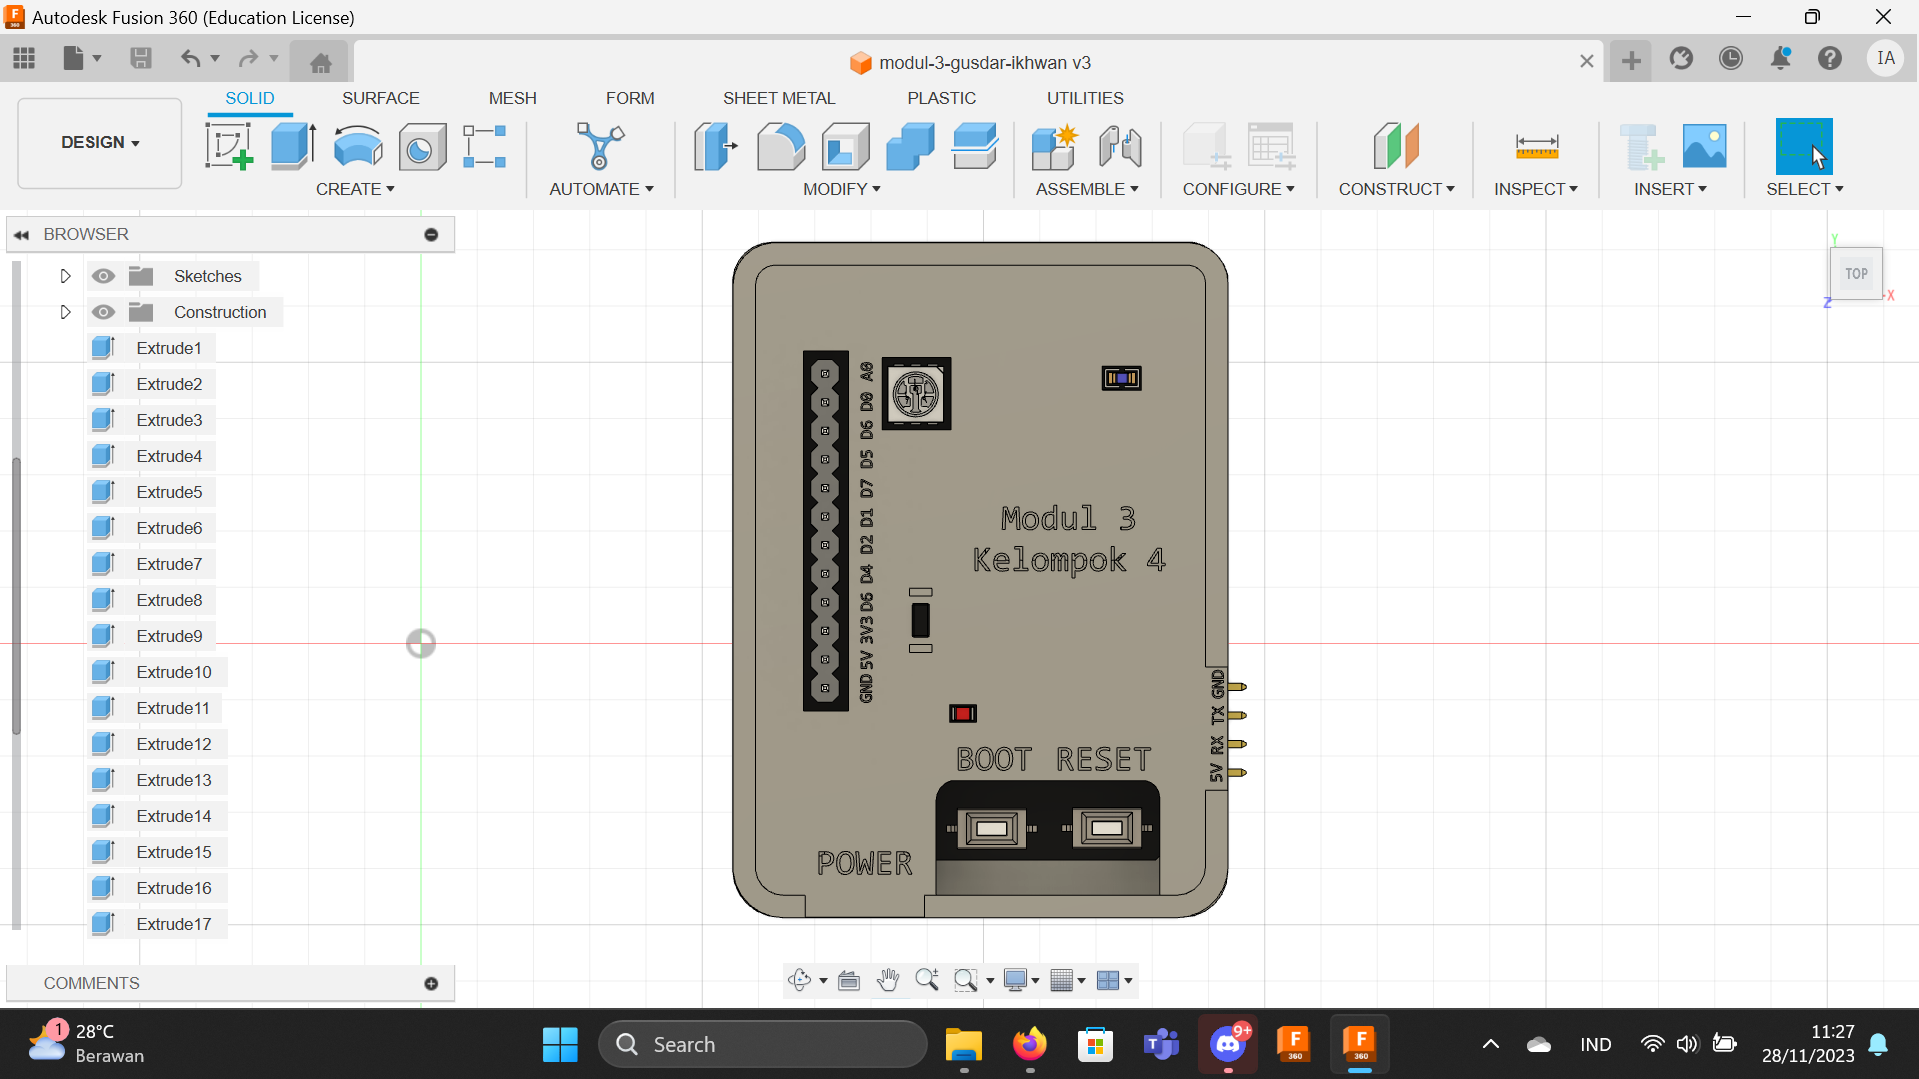
\includegraphics[width=0.8\linewidth]{img/enclosure-atas.png}
  \caption{Desain \textit{enclosure} ESP8266} 
  \label{fig:enclosure-atas}
\end{figure}

\begin{figure}[htbp]
  \centering
  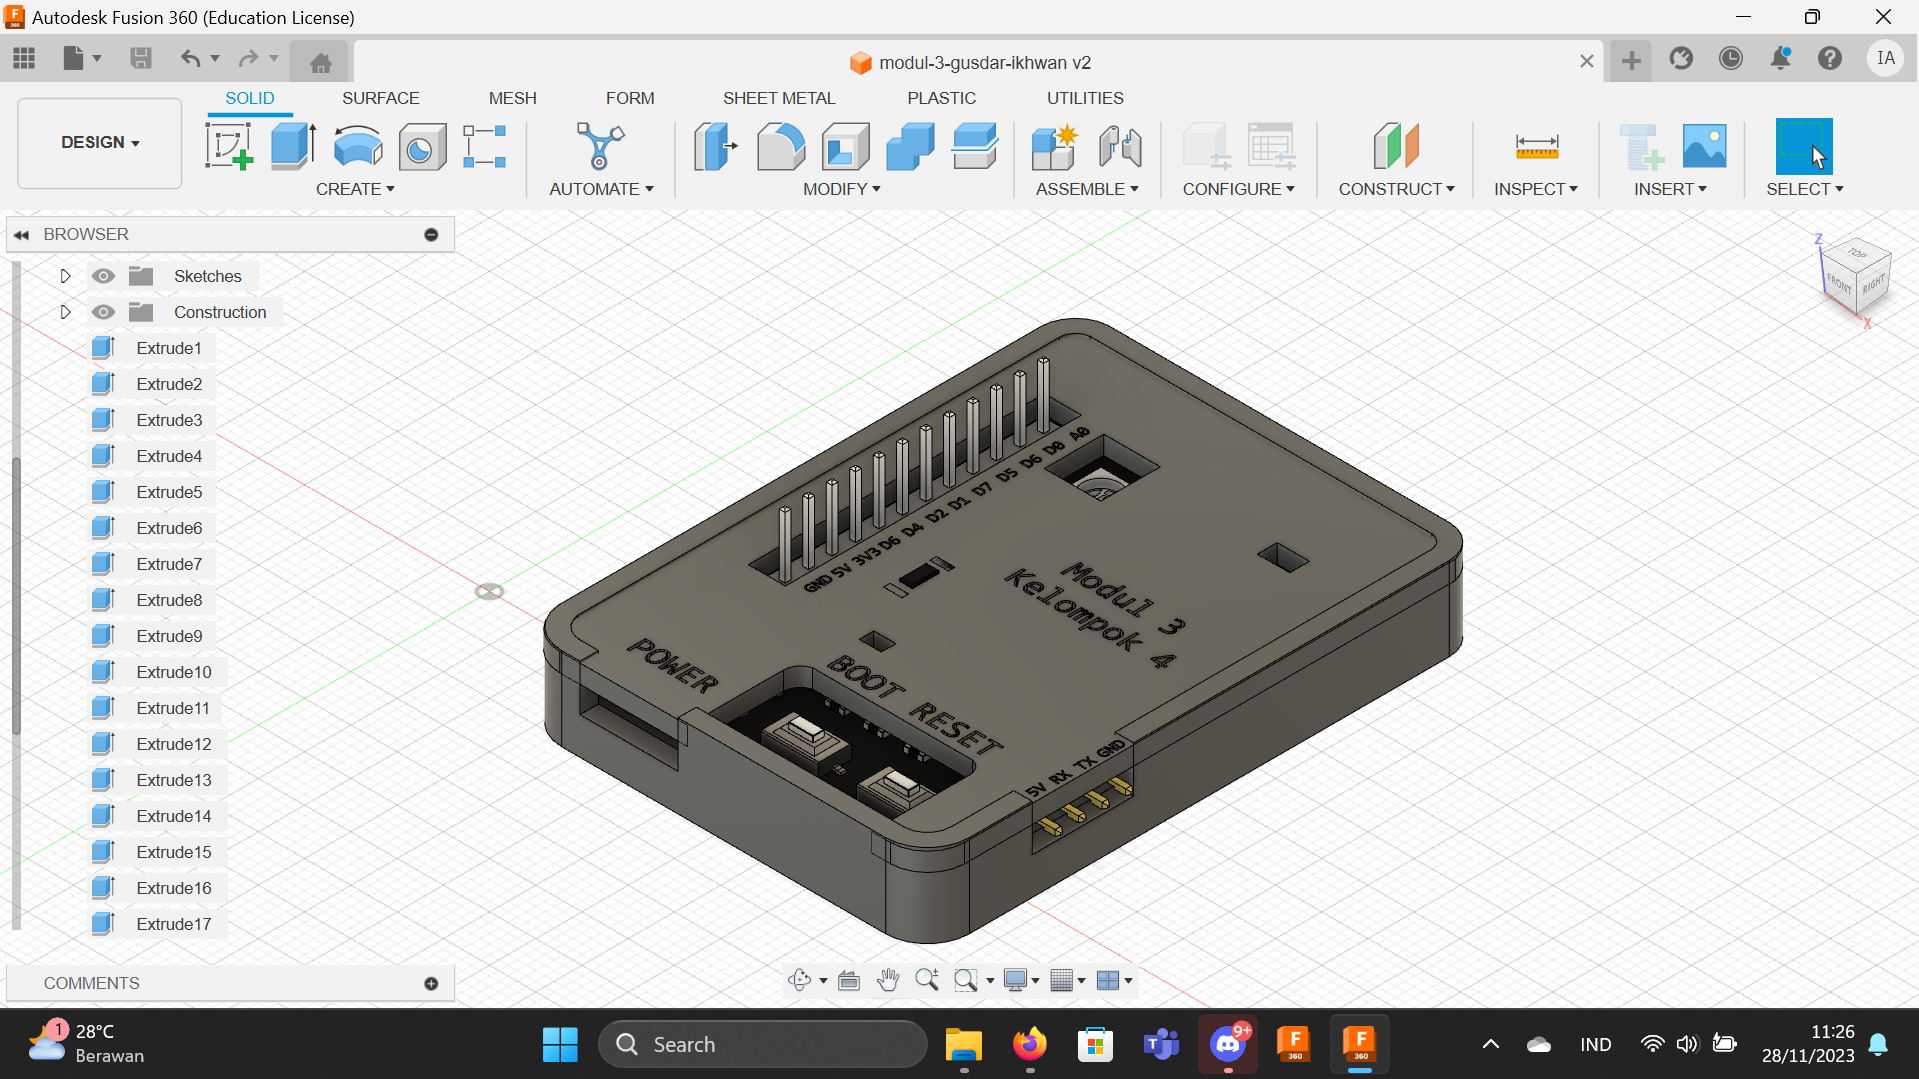
\includegraphics[width=0.8\linewidth]{img/enclosure-3d.png}
  \caption{Desain \textit{enclosure} ESP8266} 
  \label{fig:enclosure-3d}
\end{figure}

\begin{figure}[htbp]
  \centering
  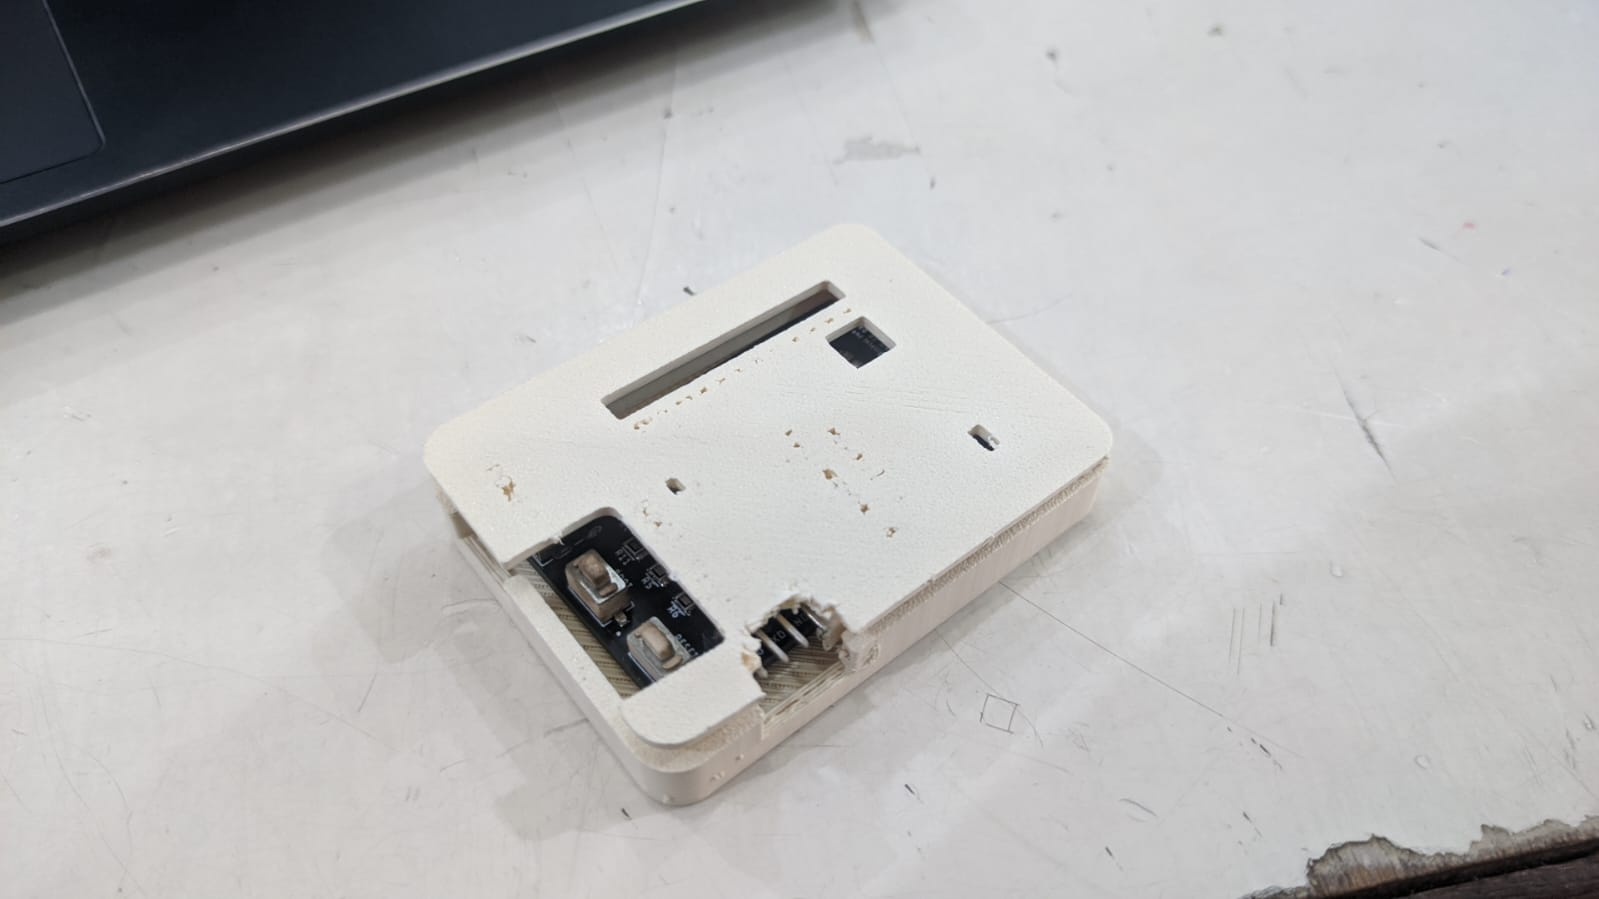
\includegraphics[width=0.8\linewidth]{img/enclosured.jpeg}
  \caption{Hasil print 3D \textit{enclosure} ESP8266} 
  \label{fig:enclosure-jadi}
\end{figure}

\begin{figure}[htbp]
  \centering
  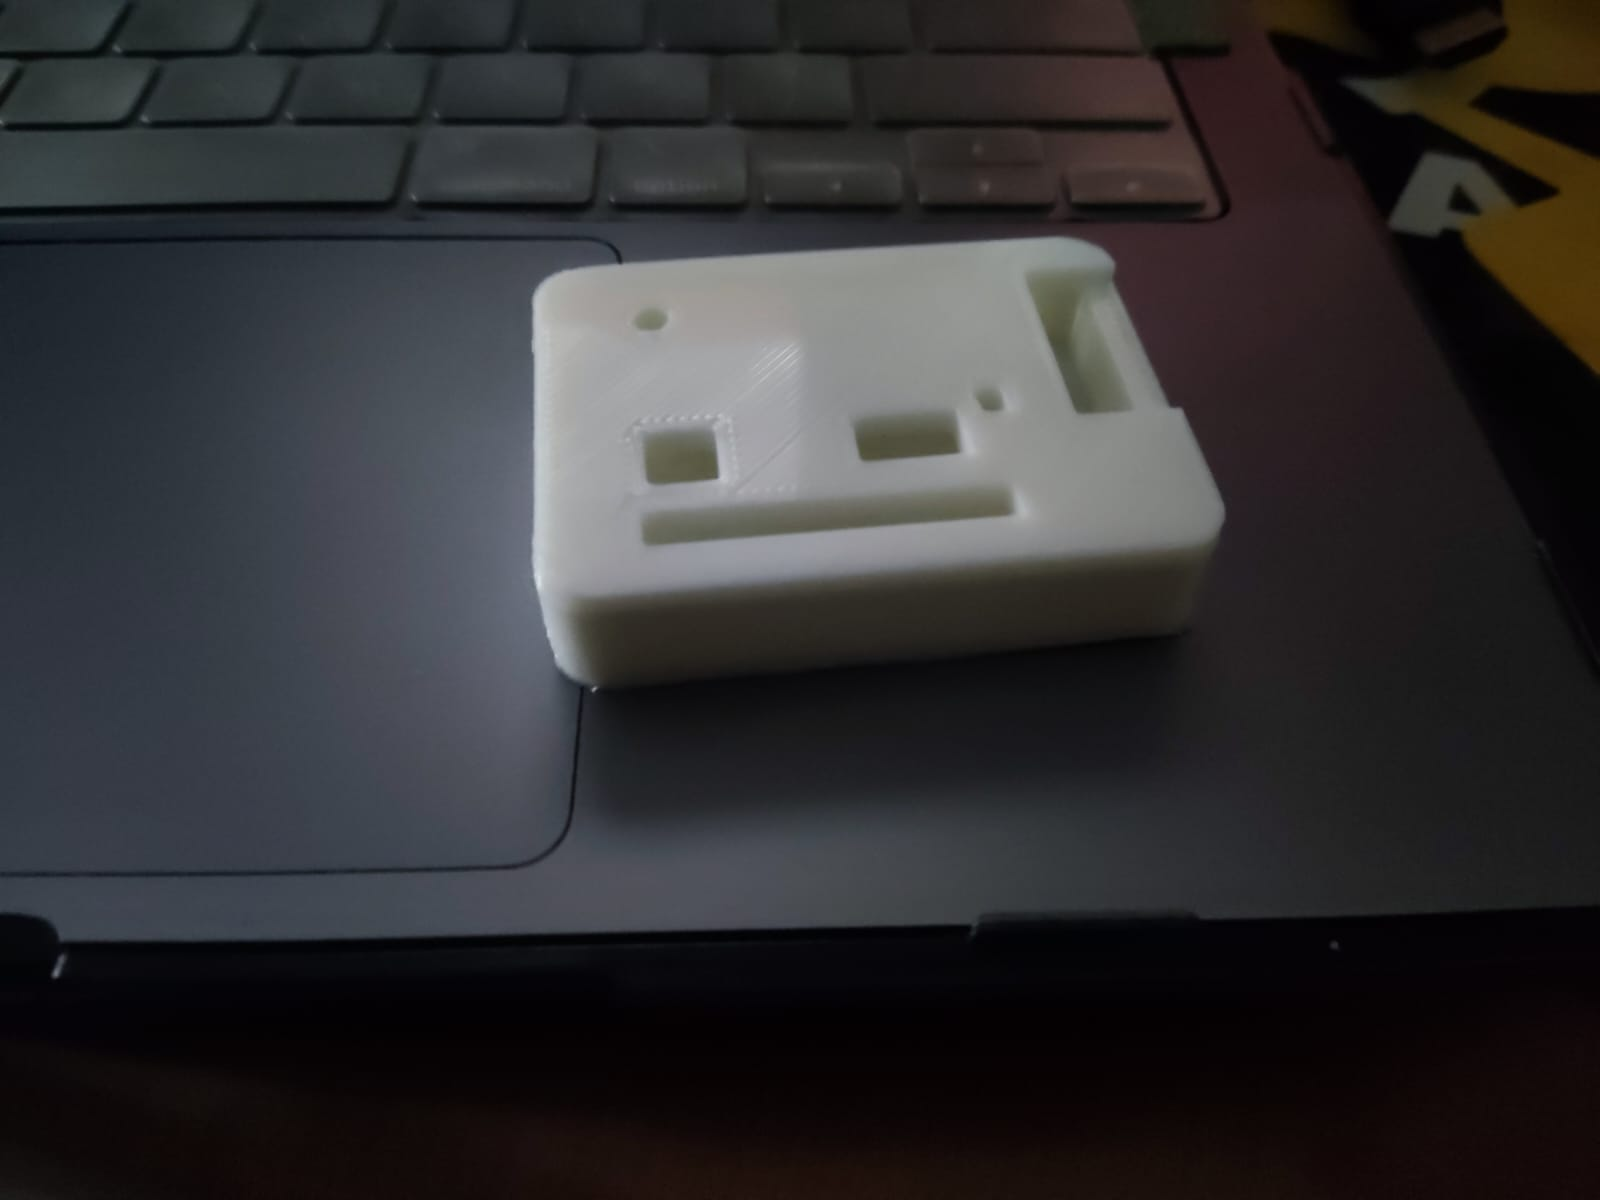
\includegraphics[width=0.8\linewidth]{img/enclosure-new.jpeg}
  \caption{Hasil print 3D ulang \textit{enclosure} ESP8266} 
  \label{fig:enclosure-jadi-new}
\end{figure}